\documentclass[tikz]{standalone}

\begin{document}
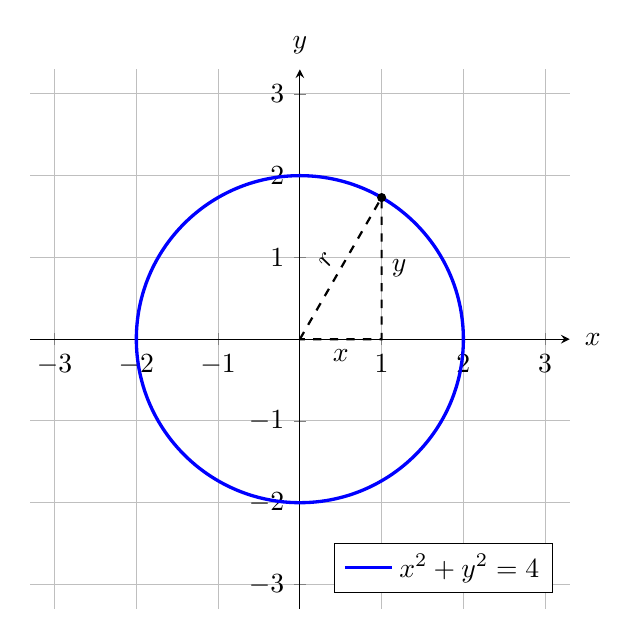
\begin{tikzpicture}
    \begin{axis}[%
        xlabel=$x$, ylabel=$y$, legend pos=south east,
        grid=both, axis lines = middle,
        minor x tick num=1, minor y tick num=1,
        xlabel style = {at={(axis description cs:1.01,0.5)},anchor=west},
        ylabel style = {at={(axis description cs:0.5,1.01)},anchor=south},
        xmin=-3.3, xmax=3.3, ymin=-3.3, ymax=3.3,
        xtick={-3,-2,-1,1,2,3}, ytick={-3,-2,-1,1,2,3},
        width=\axisdefaultwidth, height=\axisdefaultwidth,
    ]
    \addplot[very thick, blue] (0,0) circle [radius=2];
    \legend{\(x^2+y^2=4\)}
    \draw[thick, black, dashed] (0,0) -- ({2*cos(60)},{2*sin(60)}) node[above,rotate=60,midway]{$r$}
        -- ({2*cos(60)},0) node[midway,right]{$y$}
        -- cycle node[midway,below]{$x$};
    \draw[fill=black] ({2*cos(60)},{2*sin(60)}) circle (.5mm);
    \end{axis}
\end{tikzpicture}
\end{document}
